\section{Implementierung}
%\vspace{3mm}
%\begin{figure}[H]
%	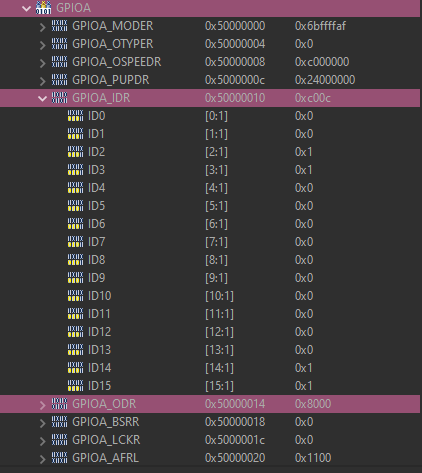
\includegraphics[width=\textwidth]{stm32_c031c6_clean_registers_setPin.PNG}
%	\caption{Register beim setzen des Pin.}
%	\label{fig:stm32_register_setPin}
%\end{figure}
%
%\vspace{3mm}
%\begin{figure}[H]
%	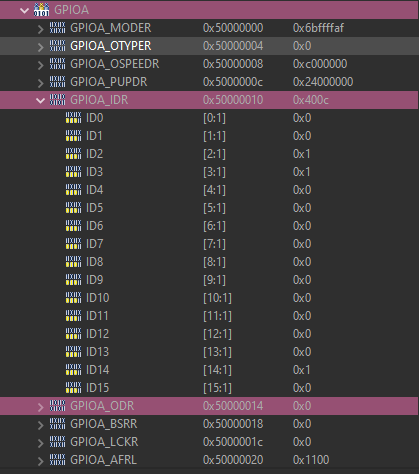
\includegraphics[width=\textwidth]{stm32_c031c6_clean_registers_resetPin.PNG}
%	\caption{Register beim zurücksetzen des Pin.}
%	\label{fig:stm32_register_resetPin}
%\end{figure}
%
%In den Abbildungen \autoref{fig:stm32_register_setPin} und \autoref{fig:stm32_register_resetPin} ist der Wert von Pin 15 (ID15 \& OD15) zu beobachten. Bei \texttt{0x0} wird der Pin zurückgesetzt und die LED leuchtet nicht mehr. Bei \texttt{0x1} wird der Wert auf $1$ gesetzt und die LED beginnt zu leuchten.
%
%Die Funktionen \texttt{HAL\_GPIO\_WritePin(GPIO\_TypeDef \*GPIOx, uint16\_t GPIO\_Pin, GPIO\_PinState PinState)} steuern nicht die in \autoref{fig:stm32_register_setPin} und \autoref{fig:stm32_register_resetPin} gezeigten Register IDR und ODR an, sondern die Set- und Reset-Register BSRR und BRR. 
%
%Diese Register sind \emph{write only}, d.h. sie können nicht ausgelesen werden.
%Wird die Funktion korrekt ausgeführt, kann dass Verhalten an den Registern IDR und ODR beobachtet werden.




